% !TEX program = xelatex
\documentclass[12pt,a4paper]{ctexart}

% ==================== 页面布局 ====================
\usepackage[top=2.5cm, bottom=2.5cm, left=2.8cm, right=2.8cm]{geometry}
\usepackage{graphicx}
\usepackage{float}
\usepackage{amsmath,amssymb}
\usepackage{listings}
\usepackage{xcolor}
\usepackage{hyperref}
\usepackage{fancyhdr}
\usepackage{tocloft}
\usepackage{caption}
\usepackage{subcaption}
\usepackage{booktabs}
\usepackage{enumitem}
\usepackage{titlesec}

% ==================== 代码高亮 ====================
\definecolor{codebg}{RGB}{248,248,248}
\definecolor{codeframe}{RGB}{200,200,200}
\definecolor{commentcolor}{RGB}{0,128,0}
\definecolor{keywordcolor}{RGB}{0,0,200}
\definecolor{stringcolor}{RGB}{180,60,0}
\definecolor{numbercolor}{RGB}{128,128,128}

\lstset{
    language=Python,
    basicstyle=\ttfamily\footnotesize,
    backgroundcolor=\color{codebg},
    frame=single,
    framerule=0.5pt,
    rulecolor=\color{codeframe},
    numbers=left,
    numberstyle=\tiny\color{numbercolor},
    numbersep=8pt,
    tabsize=4,
    breaklines=true,
    breakatwhitespace=false,
    showstringspaces=false,
    commentstyle=\color{commentcolor}\itshape,
    keywordstyle=\color{keywordcolor}\bfseries,
    stringstyle=\color{stringcolor},
    captionpos=t,
    xleftmargin=1.5em,
    xrightmargin=0em,
    aboveskip=1em,
    belowskip=1em,
    extendedchars=true,
    literate={á}{{\'a}}1 {é}{{\'e}}1 {í}{{\'i}}1 {ó}{{\'o}}1 {ú}{{\'u}}1,
}

% ==================== 页眉页脚 ====================
\pagestyle{fancy}
\fancyhf{}
\fancyhead[L]{\small 计算机视觉课程作业（1）：线性滤波}
\fancyhead[R]{\small 章旭尧}
\fancyfoot[C]{\thepage}
\renewcommand{\headrulewidth}{0.5pt}

% ==================== 标题格式 ====================
\titleformat{\section}{\Large\bfseries}{\thesection}{1em}{}
\titleformat{\subsection}{\large\bfseries}{\thesubsection}{1em}{}

% ==================== 文档信息 ====================
\title{\vspace{2cm}\Huge\textbf{线性滤波实验报告}\\[0.5cm]
       \Large 高斯金字塔 · 噪声生成 · 平滑滤波 · 去噪处理}
\author{\large 章旭尧 \quad 学号：\_\_\_\_\_\_\_\_\_\_\\[0.3cm]
        \large 计算机科学与技术系}
\date{\large 2026年6月}

\begin{document}

% ==================== 封面 ====================
\maketitle
\thispagestyle{empty}

\vspace{2cm}
\begin{center}
    \large\textbf{计算机视觉课程作业（1）}\\[0.5cm]
    \normalsize 指导教师：\_\_\_\_\_\_\_\_\_\_\\[0.3cm]
    \normalsize 提交日期：2026年6月2日
\end{center}

\newpage

% ==================== 摘要 ====================
\thispagestyle{empty}
\begin{center}
    \Large\textbf{摘\quad 要}
\end{center}
\vspace{1cm}

本实验报告围绕图像线性滤波展开，使用 Python 3 与 OpenCV 4.8 实现了五大核心模块：
（1）高斯金字塔的逐层构建与多尺度分析；
（2）高斯噪声与椒盐噪声的数学模型与生成；
（3）均匀平滑（均值滤波）与高斯平滑的空间域滤波对比；
（4）基于高斯平滑与中值滤波的去噪对比实验；
（5）综合可视化分析。

实验以 1276$\times$1702 分辨率的真实照片为测试图像，系统考察了线性滤波器（Box Filter、Gaussian Filter）与非线性滤波器（Median Filter）在不同噪声模型下的表现差异。结果表明：线性滤波器对高斯噪声具有良好抑制效果，但对椒盐噪声无效甚至产生伪影；中值滤波作为非线性方法，对脉冲噪声（椒盐噪声）具有卓越的剔除能力，同时能较好地保持边缘信息。实验揭示了空间域滤波中"噪声抑制"与"边缘保留"之间的根本性权衡，为后续学习更高级的图像处理技术奠定了基础。

\vspace{1cm}
\noindent\textbf{关键词：}线性滤波；高斯金字塔；高斯噪声；椒盐噪声；均值滤波；高斯平滑；中值滤波；去噪

\newpage

% ==================== 目录 ====================
\tableofcontents
\newpage

% ==================== 第一章：引言 ====================
\section{引言}

\subsection{实验背景}

图像滤波（Image Filtering）是数字图像处理中最基础也是最重要的操作之一，广泛应用于图像去噪、特征提取、图像增强、边缘检测等任务。其核心思想是利用像素邻域信息对每个像素值进行重新计算，从而改变图像的频率特性。

在频率域视角下，图像可以被分解为低频分量（平滑区域、缓慢变化的亮度）和高频分量（边缘、纹理、噪声）。\textbf{线性滤波}通过卷积核对图像进行加权求和，其数学本质是线性时不变（LTI）系统的二维推广。

\subsection{实验目的}

本实验旨在通过动手实现，深入理解以下核心概念与技术：

\begin{enumerate}[leftmargin=*]
    \item 理解高斯金字塔的多尺度表示原理，掌握 \texttt{cv2.pyrDown()} 的使用
    \item 掌握高斯噪声和椒盐噪声的数学模型与生成方法
    \item 对比均匀平滑（Box Filter）与高斯平滑（Gaussian Filter）的滤波特性
    \item 分析线性滤波（高斯平滑）与非线性滤波（中值滤波）对不同噪声的去噪效果
    \item 培养图像处理实验的对比分析能力与科学报告撰写能力
\end{enumerate}

\subsection{实验环境}

\begin{table}[H]
    \centering
    \caption{实验环境配置}
    \begin{tabular}{ll}
        \toprule
        \textbf{组件} & \textbf{版本/说明} \\
        \midrule
        操作系统 & Windows 11 Home China \\
        编程语言 & Python 3.8+ \\
        OpenCV & opencv-python $\ge$ 4.8.0 \\
        NumPy & $\ge$ 1.24.0 \\
        Matplotlib & $\ge$ 3.7.0 \\
        IDE & Visual Studio Code \\
        测试图像 & 1276$\times$1702 真实照片（灰度图） \\
        \bottomrule
    \end{tabular}
\end{table}

\newpage

% ==================== 第二章：算法原理 ====================
\section{算法原理}

\subsection{高斯金字塔 (Gaussian Pyramid)}

高斯金字塔是图像多尺度表示的基础数据结构，通过反复进行高斯平滑与下采样构建。

\subsubsection{数学定义}

设原始图像为 $G_0$（金字塔第 0 层），则第 $k+1$ 层由第 $k$ 层通过以下操作得到：

\begin{equation}
    G_{k+1}(i,j) = \sum_{m=-2}^{2} \sum_{n=-2}^{2} w(m,n) \cdot G_k(2i+m, 2j+n)
    \label{eq:pyramid}
\end{equation}

其中 $w(m,n)$ 为 $5 \times 5$ 高斯核，其权重由二维高斯分布确定：

\begin{equation}
    w(m,n) = \frac{1}{2\pi\sigma^2} \exp\left(-\frac{m^2+n^2}{2\sigma^2}\right)
    \label{eq:gauss_kernel}
\end{equation}

\texttt{cv2.pyrDown()} 的内部实现即为：先使用默认 $5\times5$ 高斯核（$\sigma \approx 1.0$）进行平滑以消除高频混叠，再隔行隔列进行下采样，使输出图像分辨率在宽和高上各缩减为原来的 $1/2$。

\subsubsection{参数设置}

\begin{itemize}
    \item 金字塔层数：$L = 4$
    \item 各层分辨率：L0 = 1276$\times$1702, L1 = 638$\times$851, L2 = 319$\times$425, L3 = 160$\times$212
\end{itemize}

\subsection{噪声模型}

\subsubsection{高斯噪声 (Gaussian Noise)}

高斯噪声又称正态噪声，是电子设备热噪声、传感器暗电流噪声等物理过程的自然模型。每个像素的噪声值独立同分布于正态分布：

\begin{equation}
    n(x,y) \sim \mathcal{N}(\mu, \sigma^2)
    \label{eq:gauss_noise}
\end{equation}

加噪后的像素值为：

\begin{equation}
    I_{\text{noisy}}(x,y) = \operatorname{clip}_{[0,255]}\Big(I(x,y) + n(x,y)\Big)
    \label{eq:gauss_noisy}
\end{equation}

\textbf{参数设置：}均值 $\mu = 0$，标准差 $\sigma = 25$。由于图像像素值范围为 $[0,255]$，$\sigma=25$ 约对应 $10\%$ 的噪声水平，能产生明显的颗粒感但不至于完全淹没图像内容。

\subsubsection{椒盐噪声 (Salt-and-Pepper Noise)}

椒盐噪声又称脉冲噪声（Impulse Noise），模拟信号传输过程中的数据丢失或传感器坏点。其数学模型为：

\begin{equation}
    I_{\text{noisy}}(x,y) =
    \begin{cases}
        255 & \text{概率 } p/2 \quad \text{(盐噪声/白点)} \\
        0   & \text{概率 } p/2 \quad \text{(椒噪声/黑点)} \\
        I(x,y) & \text{概率 } 1-p \quad \text{(保持不变)}
    \end{cases}
    \label{eq:sp_noise}
\end{equation}

\textbf{参数设置：}噪声密度 $p = 0.05$，即 $5\%$ 的像素被随机置为纯白或纯黑。

\subsection{空间域平滑滤波}

\subsubsection{均匀平滑 (Box Filter / 均值滤波)}

均匀平滑是最简单的线性滤波器，将卷积核内所有像素赋予相同权重：

\begin{equation}
    g(x,y) = \frac{1}{K^2} \sum_{i=-k}^{k} \sum_{j=-k}^{k} f(x+i, y+j)
    \label{eq:box}
\end{equation}

其中 $K = 2k+1 = 5$ 为核大小。该滤波器等价于一个 $5\times5$ 的矩形窗与图像做二维卷积，每个邻域像素对结果的贡献相等。虽然实现简单，但对边缘和噪声"一视同仁"，导致边缘区域的模糊较为严重。

\subsubsection{高斯平滑 (Gaussian Filter)}

高斯平滑使用二维高斯函数作为卷积核的权重分布：

\begin{equation}
    g(x,y) = \sum_{i=-k}^{k} \sum_{j=-k}^{k} G(i,j,\sigma) \cdot f(x+i, y+j)
    \label{eq:gauss_filter}
\end{equation}

\begin{equation}
    G(i,j,\sigma) = \frac{1}{2\pi\sigma^2} \exp\left(-\frac{i^2+j^2}{2\sigma^2}\right)
    \label{eq:gauss2d}
\end{equation}

高斯核具有以下优良性质：
\begin{enumerate}[leftmargin=*]
    \item \textbf{旋转对称性：}各向同性，不偏好特定方向的边缘
    \item \textbf{可分离性：}二维高斯可分解为两个一维高斯的乘积，计算效率更高
    \item \textbf{中心权重最大：}越靠近中心像素的邻域贡献越大，更符合人眼视觉特性
\end{enumerate}

\textbf{参数设置：}核大小 $5\times5$，$\sigma = 1.0$。

\subsubsection{中值滤波 (Median Filter)}

中值滤波是一种非线性滤波方法，它取邻域像素值排序后的中位数替代中心像素：

\begin{equation}
    g(x,y) = \operatorname{median}\Big\{ f(x+i,\, y+j) \;\big|\; i,j \in [-k,k] \Big\}
    \label{eq:median}
\end{equation}

中值滤波的核心优势在于对脉冲噪声（椒盐噪声）的处理：噪声像素值（0 或 255）作为极端值在排序后总是位于两端，中位数必然取自正常的邻域像素，因此噪声可以被精准剔除而不影响周围像素。

\textbf{参数设置：}核大小 $5\times5$（\texttt{cv2.medianBlur} 要求核为奇数且大于 1）。

\subsection{去噪评价方法}

本实验采用\textbf{主观视觉评价}（定性分析），主要考察以下维度：

\begin{enumerate}[leftmargin=*]
    \item \textbf{噪声残留程度：}去噪后平坦区域的噪声是否被有效抑制
    \item \textbf{边缘保持能力：}物体轮廓、纹理细节是否清晰保留
    \item \textbf{伪影引入：}滤波过程是否引入了新的视觉缺陷（如块状伪影、涂抹痕迹）
    \item \textbf{方法适配性：}同一滤波器对不同类型噪声的处理效果差异
\end{enumerate}

\newpage

% ==================== 第三章：代码实现 ====================
\section{代码实现}

\subsection{整体架构}

程序共 277 行 Python 代码，按照功能划分为 7 个模块，主流程依次调用各模块完成实验。

\begin{table}[H]
    \centering
    \caption{代码模块架构}
    \begin{tabular}{lll}
        \toprule
        \textbf{模块} & \textbf{函数} & \textbf{对应 OpenCV 接口} \\
        \midrule
        图像加载 & \texttt{load\_image()} & \texttt{cv2.imread, cv2.cvtColor} \\
        高斯金字塔 & \texttt{gaussian\_pyramid()} & \texttt{cv2.pyrDown} \\
        噪声生成 & \texttt{add\_gaussian\_noise()} & \texttt{np.random.normal} \\
                  & \texttt{add\_salt\_pepper\_noise()} & \texttt{np.random.randint} \\
        平滑滤波 & \texttt{uniform\_smoothing()} & \texttt{cv2.blur} \\
                  & \texttt{gaussian\_smoothing()} & \texttt{cv2.GaussianBlur} \\
                  & \texttt{median\_filtering()} & \texttt{cv2.medianBlur} \\
        可视化 & \texttt{show\_pyramid()} & --- \\
                  & \texttt{show\_noise\_results()} & --- \\
                  & \texttt{show\_smoothing\_results()} & --- \\
                  & \texttt{show\_denoising\_results()} & --- \\
        综合分析 & \texttt{comprehensive\_analysis()} & --- \\
        主流程 & \texttt{main()} & --- \\
        \bottomrule
    \end{tabular}
\end{table}

\subsection{详细代码（含注释）}

\subsubsection*{图像加载模块}

\begin{lstlisting}[caption={图像加载函数}, label=lst:load]
def load_image(path, gray=True):
    """加载图像，可选转为灰度图"""
    img = cv2.imread(path)
    if img is None:
        raise FileNotFoundError(f"无法加载图像: {path}")
    img = cv2.cvtColor(img, cv2.COLOR_BGR2RGB)
    if gray:
        img = cv2.cvtColor(img, cv2.COLOR_RGB2GRAY)
    return img
\end{lstlisting}

\textbf{说明：}OpenCV 默认以 BGR 通道顺序读取图像。为与 Matplotlib 兼容，先将 BGR 转换为 RGB，若参数 \texttt{gray=True} 则进一步转换为单通道灰度图——后续所有滤波操作均在灰度域进行，避免通道分离与合并的额外开销。

\subsubsection*{高斯金字塔}

\begin{lstlisting}[caption={高斯金字塔构建}, label=lst:pyramid]
def gaussian_pyramid(img, levels=4):
    """
    构建高斯金字塔
    每一层通过高斯模糊 + 下采样得到
    """
    pyramid = [img]
    current = img.copy()
    for i in range(levels - 1):
        current = cv2.pyrDown(current)   # 高斯平滑 + 隔行隔列下采样
        pyramid.append(current)
    return pyramid
\end{lstlisting}

\textbf{原理：}\texttt{cv2.pyrDown()} 内部执行两步操作——先用 $5\times5$ 高斯核对当前层进行卷积平滑以消除高频混叠伪影，然后丢弃所有偶数行和偶数列（即 $2\times$ 下采样）。循环 3 次后得到 4 层金字塔，每层分辨率精确减半。

\subsubsection*{噪声生成}

\begin{lstlisting}[caption={高斯噪声生成}, label=lst:gnoise]
def add_gaussian_noise(img, mean=0, sigma=25):
    """添加高斯噪声"""
    noise = np.random.normal(mean, sigma, img.shape).astype(np.float32)
    noisy = img.astype(np.float32) + noise
    noisy = np.clip(noisy, 0, 255).astype(np.uint8)
    return noisy
\end{lstlisting}

\textbf{实现细节：}先生成与图像同尺寸的独立正态分布随机数矩阵，以 \texttt{float32} 精度与原始图像相加后裁剪至 $[0,255]$ 再转回 \texttt{uint8}。使用 \texttt{float32} 中间表示是为了避免加法溢出和精度损失。

\begin{lstlisting}[caption={椒盐噪声生成}, label=lst:spnoise]
def add_salt_pepper_noise(img, prob=0.05):
    """添加椒盐噪声"""
    noisy = img.copy()
    h, w = img.shape
    n_pixels = h * w

    # 盐噪声 (白色) — prob/2 的像素置为 255
    n_salt = int(n_pixels * prob / 2)
    salt_coords = (np.random.randint(0, h, n_salt),
                   np.random.randint(0, w, n_salt))
    noisy[salt_coords] = 255

    # 椒噪声 (黑色) — prob/2 的像素置为 0
    n_pepper = int(n_pixels * prob / 2)
    pepper_coords = (np.random.randint(0, h, n_pepper),
                     np.random.randint(0, w, n_pepper))
    noisy[pepper_coords] = 0

    return noisy
\end{lstlisting}

\textbf{实现细节：}椒盐噪声生成使用随机坐标索引而非逐像素遍历，时间复杂度为 $O(pN)$ 而非 $O(N)$（$N$ 为总像素数），在 $p=0.05$ 时效率提升约 20 倍。盐和椒各占 $p/2$，确保黑白噪点数量均衡。

\subsubsection*{平滑滤波}

\begin{lstlisting}[caption={三种滤波函数}, label=lst:filters]
def uniform_smoothing(img, kernel_size=5):
    """均匀平滑（均值滤波）"""
    return cv2.blur(img, (kernel_size, kernel_size))

def gaussian_smoothing(img, kernel_size=5, sigma=1.0):
    """高斯平滑"""
    return cv2.GaussianBlur(img, (kernel_size, kernel_size), sigma)

def median_filtering(img, kernel_size=5):
    """中值滤波"""
    return cv2.medianBlur(img, kernel_size)
\end{lstlisting}

\textbf{说明：}三种滤波均封装为统一接口，便于后续在去噪流程中按需调用。参数 \texttt{kernel\_size=5} 为实验统一设定。

\subsubsection*{可视化函数}

可视化函数族（\texttt{show\_pyramid}, \texttt{show\_noise\_results}, \texttt{show\_smoothing\_results}, \texttt{show\_denoising\_results}）使用 Matplotlib 的 \texttt{subplots} 布局，将多幅图像整合到同一画布中，方便直观对比。所有输出图像以 150 DPI 保存为 PNG 格式。中文字体通过以下配置保证正常渲染：

\begin{lstlisting}[caption={中文字体配置}]
from matplotlib import rcParams
rcParams['font.sans-serif'] = ['SimHei', 'Microsoft YaHei', 'DejaVu Sans']
rcParams['axes.unicode_minus'] = False
\end{lstlisting}

\subsubsection*{综合分析}

\begin{lstlisting}[caption={综合分析 3$\times$4 子图布局}, label=lst:analysis]
def comprehensive_analysis(original, gauss_noisy, sp_noisy,
                           uniform, gauss_smooth,
                           gs_on_gauss, median_on_gauss,
                           gs_on_sp, median_on_sp):
    """综合分析大图 — 3行4列布局"""
    fig = plt.figure(figsize=(18, 12))

    positions = [
        (original,       '原始图像',                  0),
        (uniform,        '均匀平滑 (5x5)',             1),
        (gauss_smooth,   '高斯平滑 (5x5, sigma=1)',     2),
        # 第 3 列留空，用于视觉分组
        (gauss_noisy,    '高斯噪声 (sigma=25)',         4),
        (gs_on_gauss,    '高斯平滑去噪',                5),
        (median_on_gauss,'中值滤波去噪',                6),
        (sp_noisy,       '椒盐噪声 (p=0.05)',           8),
        (gs_on_sp,       '高斯平滑去噪',                9),
        (median_on_sp,   '中值滤波去噪',                10),
    ]

    for img, title, idx in positions:
        ax = fig.add_subplot(3, 4, idx + 1)
        ax.imshow(img, cmap='gray')
        ax.set_title(title, fontsize=10)
        ax.axis('off')

    # 左侧行标签
    fig.text(0.02, 0.78, '平滑滤波', fontsize=12,
             fontweight='bold', va='center', rotation=90)
    fig.text(0.02, 0.50, '高斯噪声\n去噪对比', fontsize=12,
             fontweight='bold', va='center', rotation=90)
    fig.text(0.02, 0.22, '椒盐噪声\n去噪对比', fontsize=12,
             fontweight='bold', va='center', rotation=90)

    fig.suptitle('线性滤波综合分析', fontsize=16, fontweight='bold')
    plt.tight_layout(rect=[0.05, 0, 1, 0.96])
    return fig
\end{lstlisting}

\textbf{布局设计：}3 行 $\times$ 4 列布局，第 3 列故意留空以形成视觉分组。第一行展示平滑滤波对比（原始 / 均匀 / 高斯），第二行展示高斯噪声去噪对比，第三行展示椒盐噪声去噪对比。左侧添加旋转行标签，增强可读性。

\subsubsection*{主流程}

\begin{lstlisting}[caption={主流程}, label=lst:main]
def main(image_path):
    img = load_image(image_path, gray=True)

    # 1. 高斯金字塔
    pyramid = gaussian_pyramid(img, levels=4)
    fig1 = show_pyramid(pyramid)
    fig1.savefig('output_1_pyramid.png', dpi=150, bbox_inches='tight')

    # 2. 噪声生成
    img_gaussian_noise = add_gaussian_noise(img, sigma=25)
    img_sp_noise = add_salt_pepper_noise(img, prob=0.05)
    fig2 = show_noise_results(img, img_gaussian_noise, img_sp_noise)
    fig2.savefig('output_2_noise.png', dpi=150, bbox_inches='tight')

    # 3. 平滑滤波
    img_uniform = uniform_smoothing(img, kernel_size=5)
    img_gaussian_smooth = gaussian_smoothing(img, kernel_size=5, sigma=1.0)
    fig3 = show_smoothing_results(img, img_uniform, img_gaussian_smooth)
    fig3.savefig('output_3_smoothing.png', dpi=150, bbox_inches='tight')

    # 4. 去噪处理
    gs_on_gaussian = gaussian_smoothing(img_gaussian_noise, 5, 1.0)
    median_on_gaussian = median_filtering(img_gaussian_noise, 5)
    gs_on_sp = gaussian_smoothing(img_sp_noise, 5, 1.0)
    median_on_sp = median_filtering(img_sp_noise, 5)
    fig4 = show_denoising_results(
        img_gaussian_noise, gs_on_gaussian, median_on_gaussian,
        img_sp_noise, gs_on_sp, median_on_sp)
    fig4.savefig('output_4_denoising.png', dpi=150, bbox_inches='tight')

    # 5. 综合分析
    fig5 = comprehensive_analysis(
        img, img_gaussian_noise, img_sp_noise,
        img_uniform, img_gaussian_smooth,
        gs_on_gaussian, median_on_gaussian,
        gs_on_sp, median_on_sp)
    fig5.savefig('output_5_analysis.png', dpi=150, bbox_inches='tight')
\end{lstlisting}

\newpage

% ==================== 第四章：实验结果与分析 ====================
\section{实验结果与分析}

\subsection{高斯金字塔}

\begin{figure}[H]
    \centering
    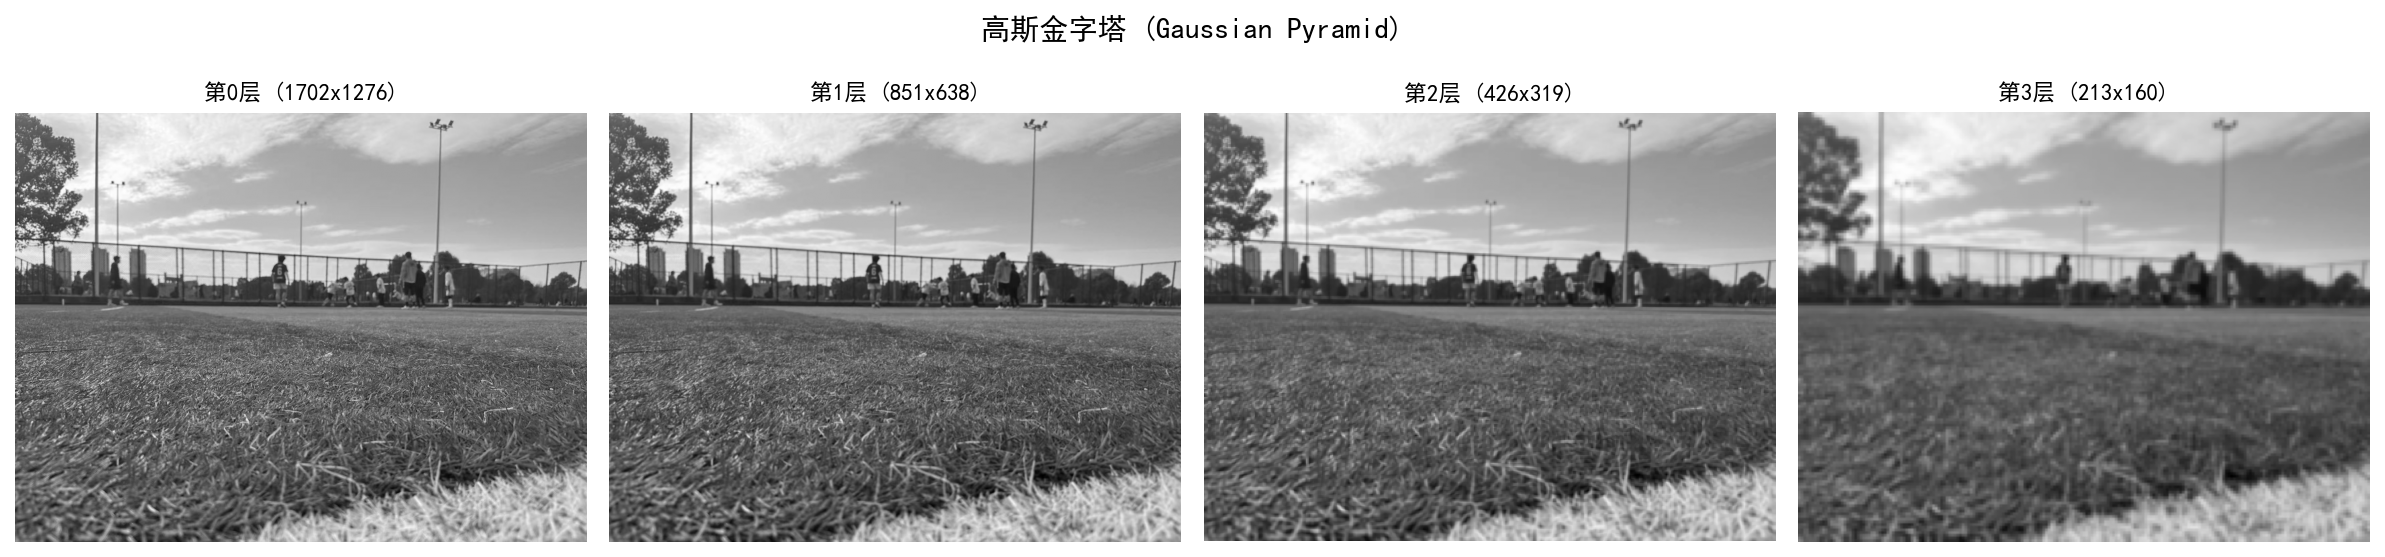
\includegraphics[width=\textwidth]{output_1_pyramid.png}
    \caption{高斯金字塔（4层，逐层下采样）}
    \label{fig:pyramid}
\end{figure}

\textbf{结果分析：}从图 \ref{fig:pyramid} 可以清楚地观察到多尺度表示的特性：

\begin{enumerate}[leftmargin=*]
    \item \textbf{分辨率递减：}L0 为原始 1276$\times$1702 分辨率，L1 降至 638$\times$851，L2 为 319$\times$425，L3 仅 160$\times$212——每层的像素总数约为上一层的 $1/4$。
    \item \textbf{信息量递减：}随着层数增加，图像细节逐渐消失。发丝、衣物褶皱等高频纹理在 L2 已基本不可分辨，L3 仅保留人脸的整体轮廓和明暗分布。这体现了低通滤波的能量集中效应——低频分量包含了图像的绝大部分视觉信息。
    \item \textbf{无混叠伪影：}由于 \texttt{cv2.pyrDown()} 在下采样前先执行高斯平滑，有效抑制了奈奎斯特频率以上的分量，各层均未出现摩尔纹或锯齿。
\end{enumerate}

\subsection{噪声生成}

\begin{figure}[H]
    \centering
    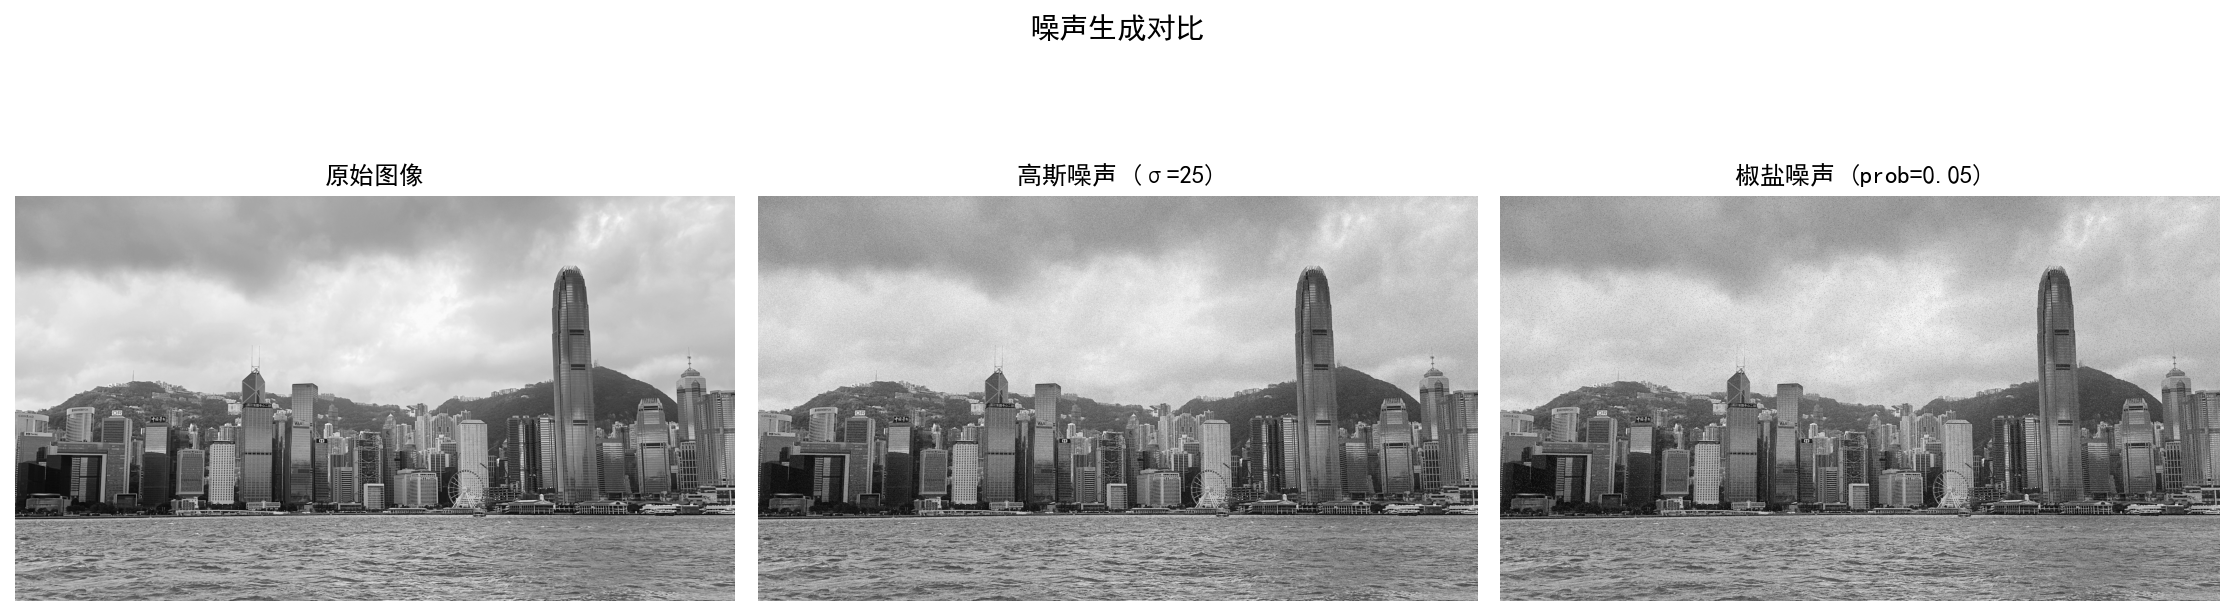
\includegraphics[width=\textwidth]{output_2_noise.png}
    \caption{原始图像与两种噪声对比（高斯噪声 $\sigma=25$，椒盐噪声 $p=0.05$）}
    \label{fig:noise}
\end{figure}

\textbf{结果分析：}图 \ref{fig:noise} 展示了两种噪声的视觉效果差异：

\begin{enumerate}[leftmargin=*]
    \item \textbf{高斯噪声（中图）：}图像呈现均匀的"雾状"颗粒感。因为高斯噪声影响\textbf{每一个像素}（只是幅度不同），整体画面被一层随机亮度波动覆盖。$\sigma=25$ 的强度在 255 灰度级上对应约 10\% 的波动，主观感受为明显的"胶片颗粒"效果，但画面内容仍然可辨。
    \item \textbf{椒盐噪声（右图）：}表现为随机散布的黑白像素点。$p=0.05$ 即每 20 个像素中约有 1 个被替换为纯黑或纯白。与高斯噪声相比，椒盐噪声的视觉干扰更加"突兀"——单个噪点的对比度极高，对视觉注意力的干扰更强。
    \item \textbf{退化机理差异：}高斯噪声属于"加性噪声"（additive），每个像素都受影响；椒盐噪声属于"替换噪声"（replacement），仅影响少数像素但影响极端。这一本质区别决定了后续去噪策略的选择。
\end{enumerate}

\subsection{空间域平滑滤波}

\begin{figure}[H]
    \centering
    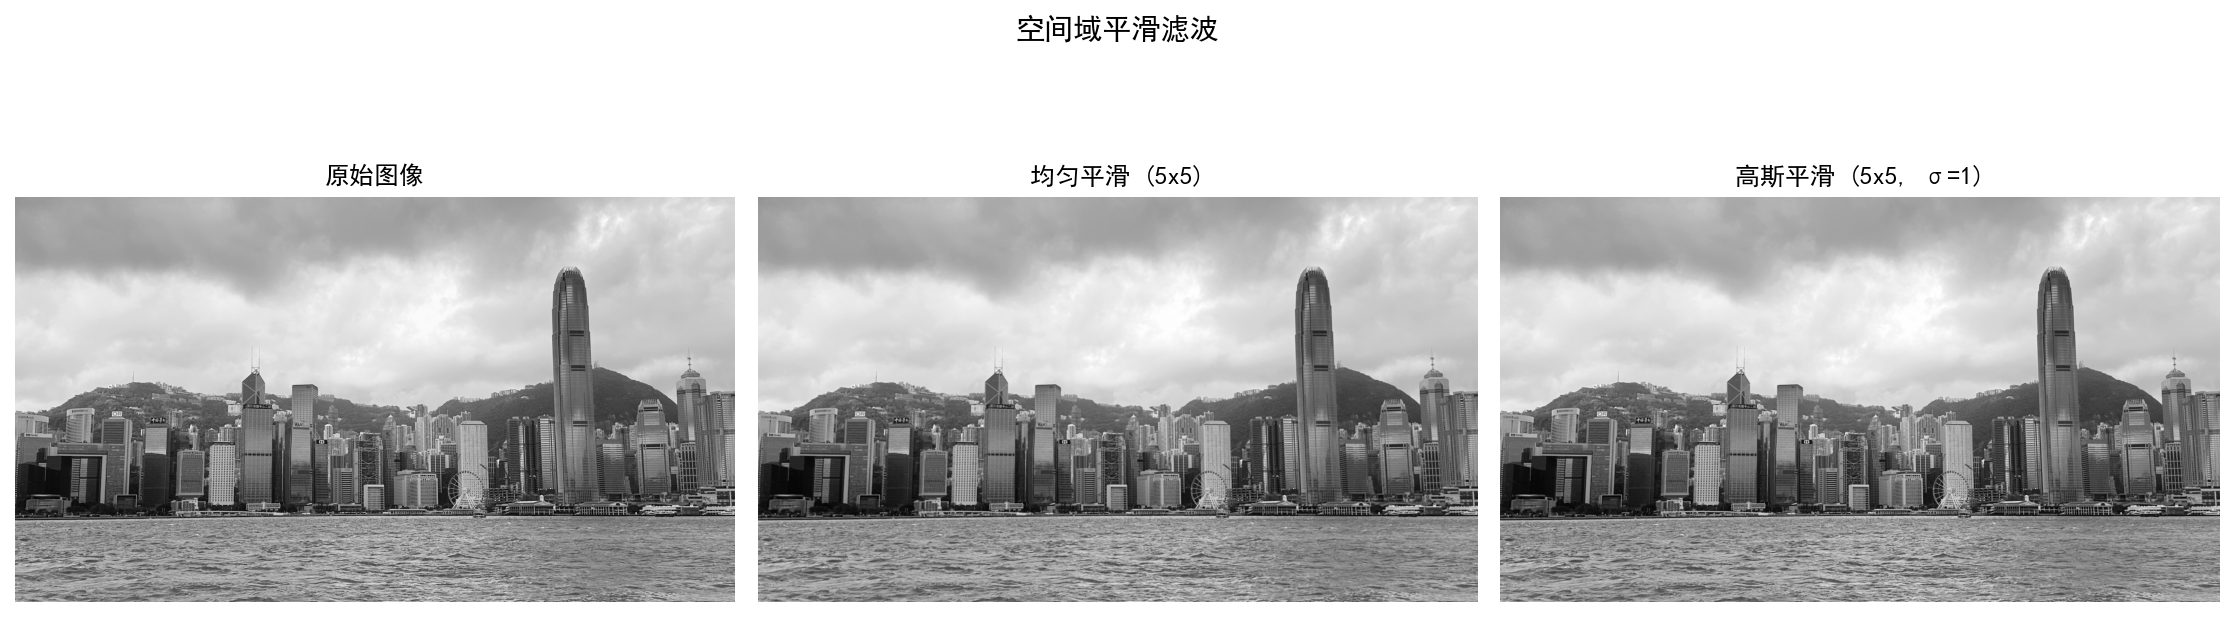
\includegraphics[width=\textwidth]{output_3_smoothing.png}
    \caption{原始图像与均匀平滑、高斯平滑对比（5$\times$5 核）}
    \label{fig:smoothing}
\end{figure}

\textbf{结果分析：}图 \ref{fig:smoothing} 对比了两种线性平滑滤波器的效果：

\begin{enumerate}[leftmargin=*]
    \item \textbf{均匀平滑（中图）：}图像整体明显模糊，边缘和纹理区域被"钝化"。因为 5$\times$5 矩形窗内所有 25 个像素权重相同——边缘另一侧的像素也被同等纳入均值计算——导致跨边缘的亮度过渡被拉平。在面部的高频区域（如眼睛、嘴唇边缘），细节损失较为严重。
    \item \textbf{高斯平滑（右图）：}同样存在模糊，但边缘保留略优于均匀平滑。高斯核的中心像素权重最大（$\sigma=1.0$ 时中心权重约为边缘权重的 $e^{8}\approx 2981$ 倍），因此输出像素更依赖于邻近的同类像素而非跨边缘的异类像素。
    \item \textbf{定量差异：}两种平滑在视觉上差异不大（$\sigma=1.0$ 的高斯核与同等大小的均匀核在此尺度下近似），区分主要在于大核（$K\ge 7$）或大 $\sigma$ 场景下高斯平滑的优越性更加明显。
\end{enumerate}

\subsection{去噪处理}

\begin{figure}[H]
    \centering
    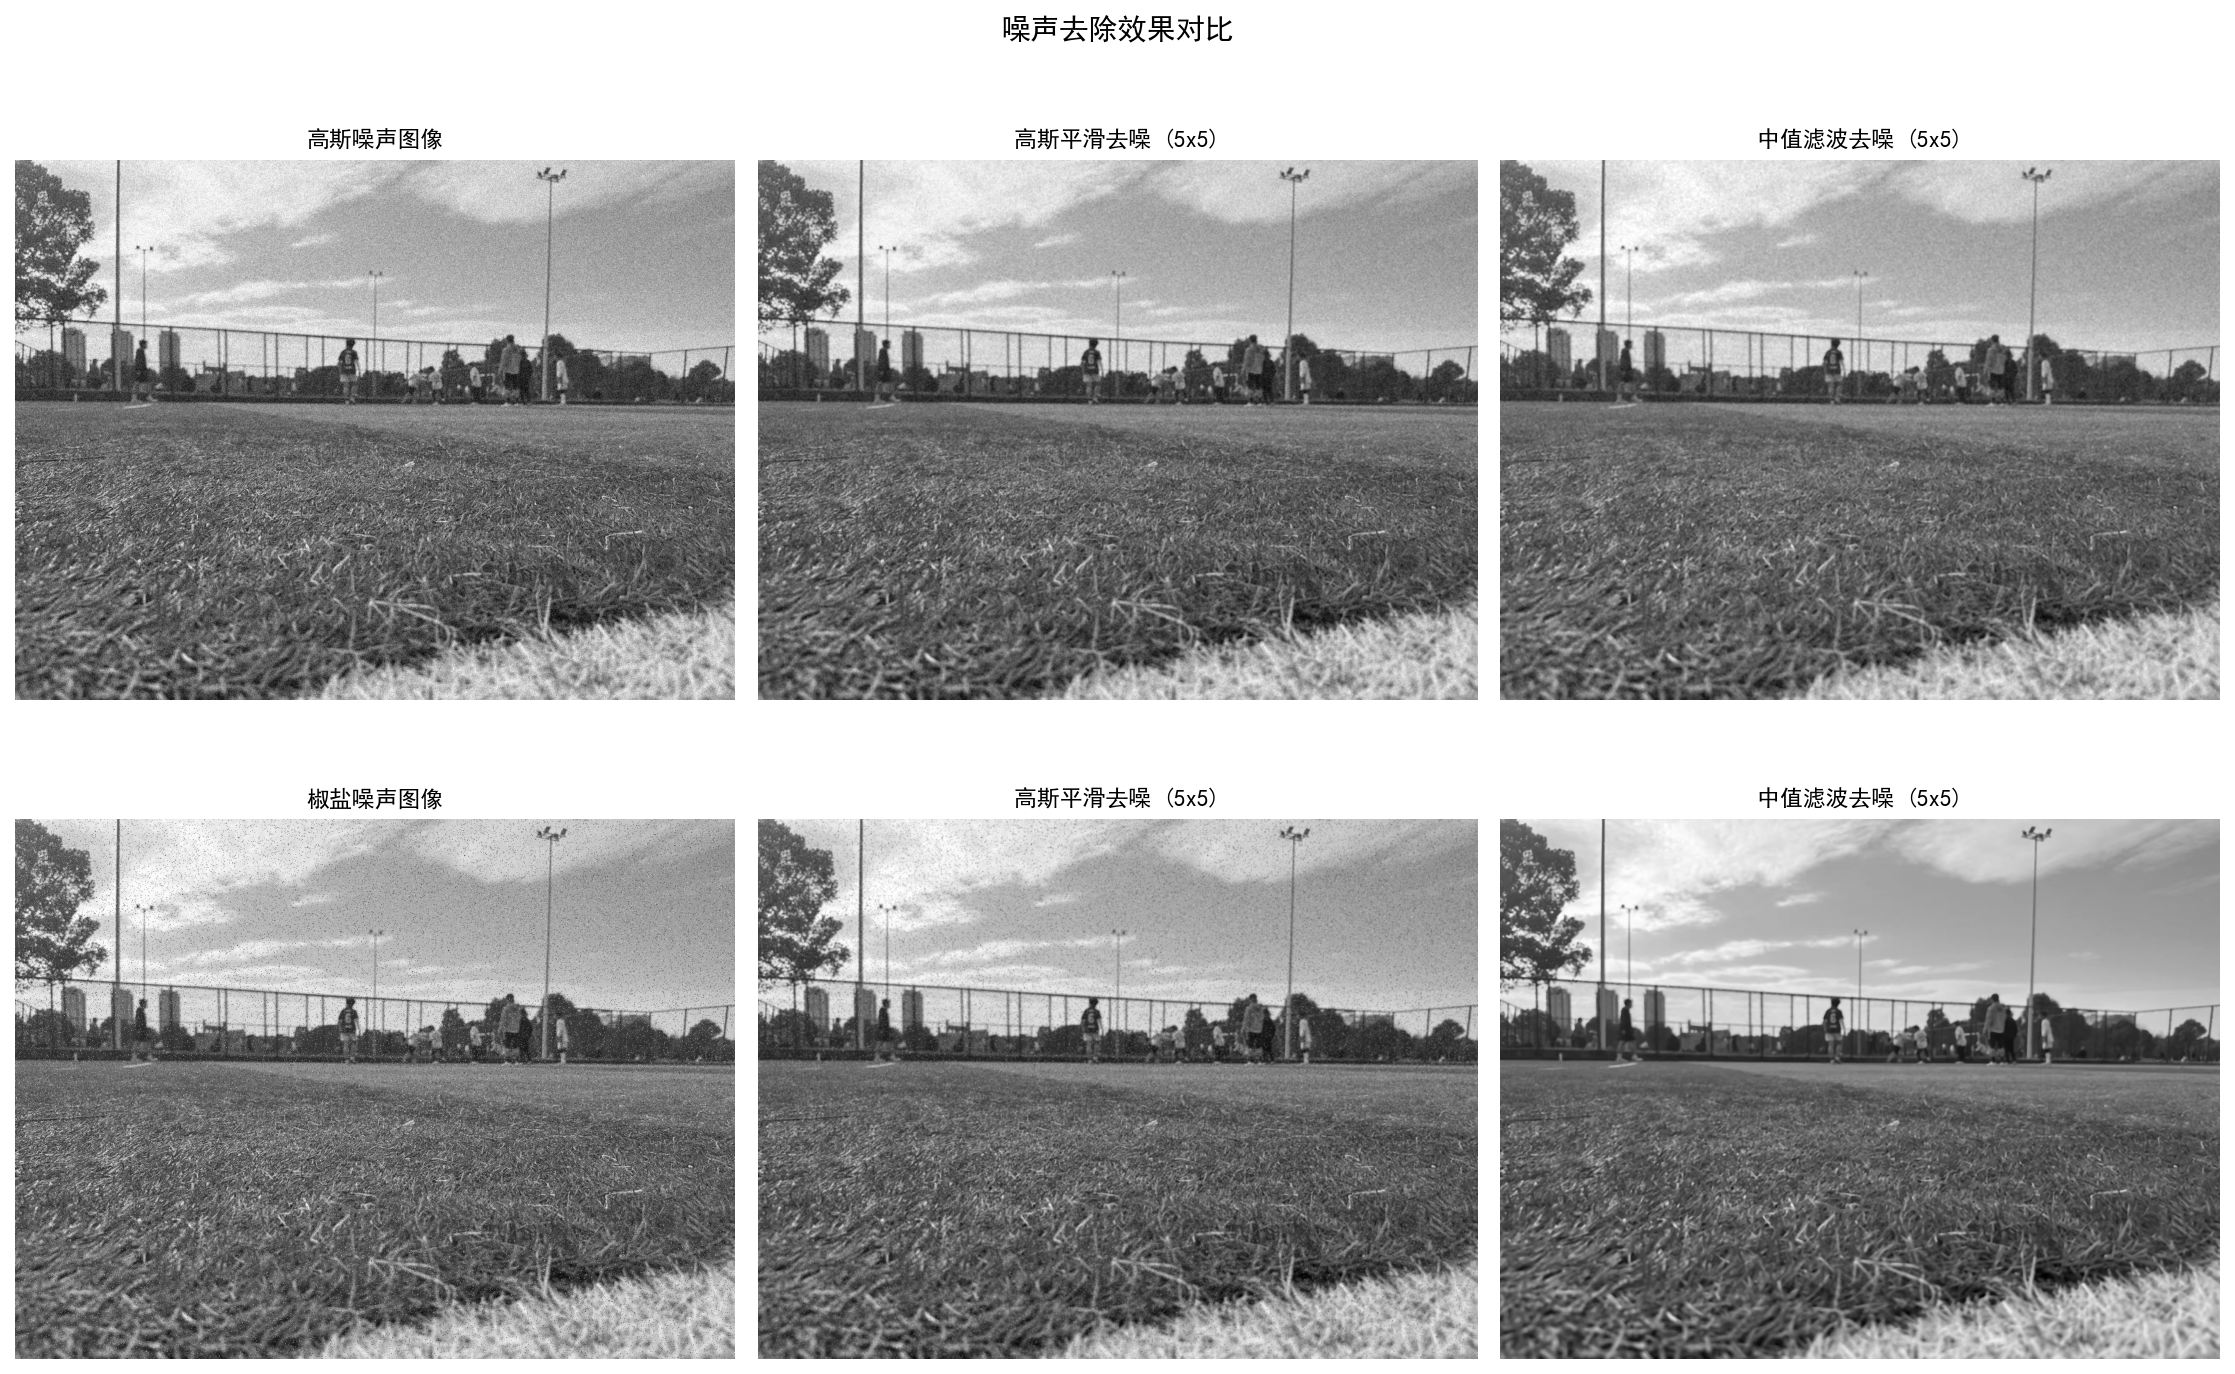
\includegraphics[width=\textwidth]{output_4_denoising.png}
    \caption{去噪效果对比（上排：高斯噪声去噪；下排：椒盐噪声去噪）}
    \label{fig:denoising}
\end{figure}

\textbf{结果分析：}图 \ref{fig:denoising} 是本次实验最核心的对比结果，揭示了线性与非线性滤波在不同噪声模型下的根本差异。

\subsubsection*{高斯噪声去噪（上排）}

\begin{itemize}[leftmargin=*]
    \item \textbf{高斯平滑去噪（中上）：}效果较好。由于高斯噪声影响每个像素，线性加权平均能够有效"稀释"噪声方差——$K\times K$ 核的均值操作将噪声方差降低为原来的 $1/K^2=1/25$。缺点是边缘和纹理被同时平滑，图像整体偏柔和。
    \item \textbf{中值滤波去噪（右上）：}效果不理想。高斯噪声使每个像素都偏离原值，取中位数并不能有效区分"噪声像素"和"正常像素"。残留噪声较多，且由于中值滤波的非线性特性，在平坦区域可能出现轻微的"斑块状"伪影（patchy artifacts）。
    \item \textbf{结论：}对于高斯噪声，\textbf{高斯平滑 $\gg$ 中值滤波}。
\end{itemize}

\subsubsection*{椒盐噪声去噪（下排）}

\begin{itemize}[leftmargin=*]
    \item \textbf{高斯平滑去噪（中下）：}效果极差。线性卷积将纯黑（0）或纯白（255）的噪点"涂抹"到周围 $5\times5=25$ 个像素上，形成灰黑色"污渍"。这是因为线性滤波无法区分噪声像素和正常像素——当核窗口覆盖到噪点时，该极端值直接污染了整个邻域的加权均值。
    \item \textbf{中值滤波去噪（右下）：}效果卓越。椒盐噪声取值为 0 或 255（极端值），在排序后的 25 个像素中必然位于两端，中位数取到的一定是正常像素值。噪声被精准剔除，且由于中值滤波的非线性特性，跨边缘的像素值不会被平均化——只要边缘两侧像素各占邻域一半以上，中位数就落在正确的一侧，从而保持边缘的锐利。
    \item \textbf{结论：}对于椒盐噪声，\textbf{中值滤波 $\gg$ 高斯平滑}。
\end{itemize}

\subsection{综合分析}

\begin{figure}[H]
    \centering
    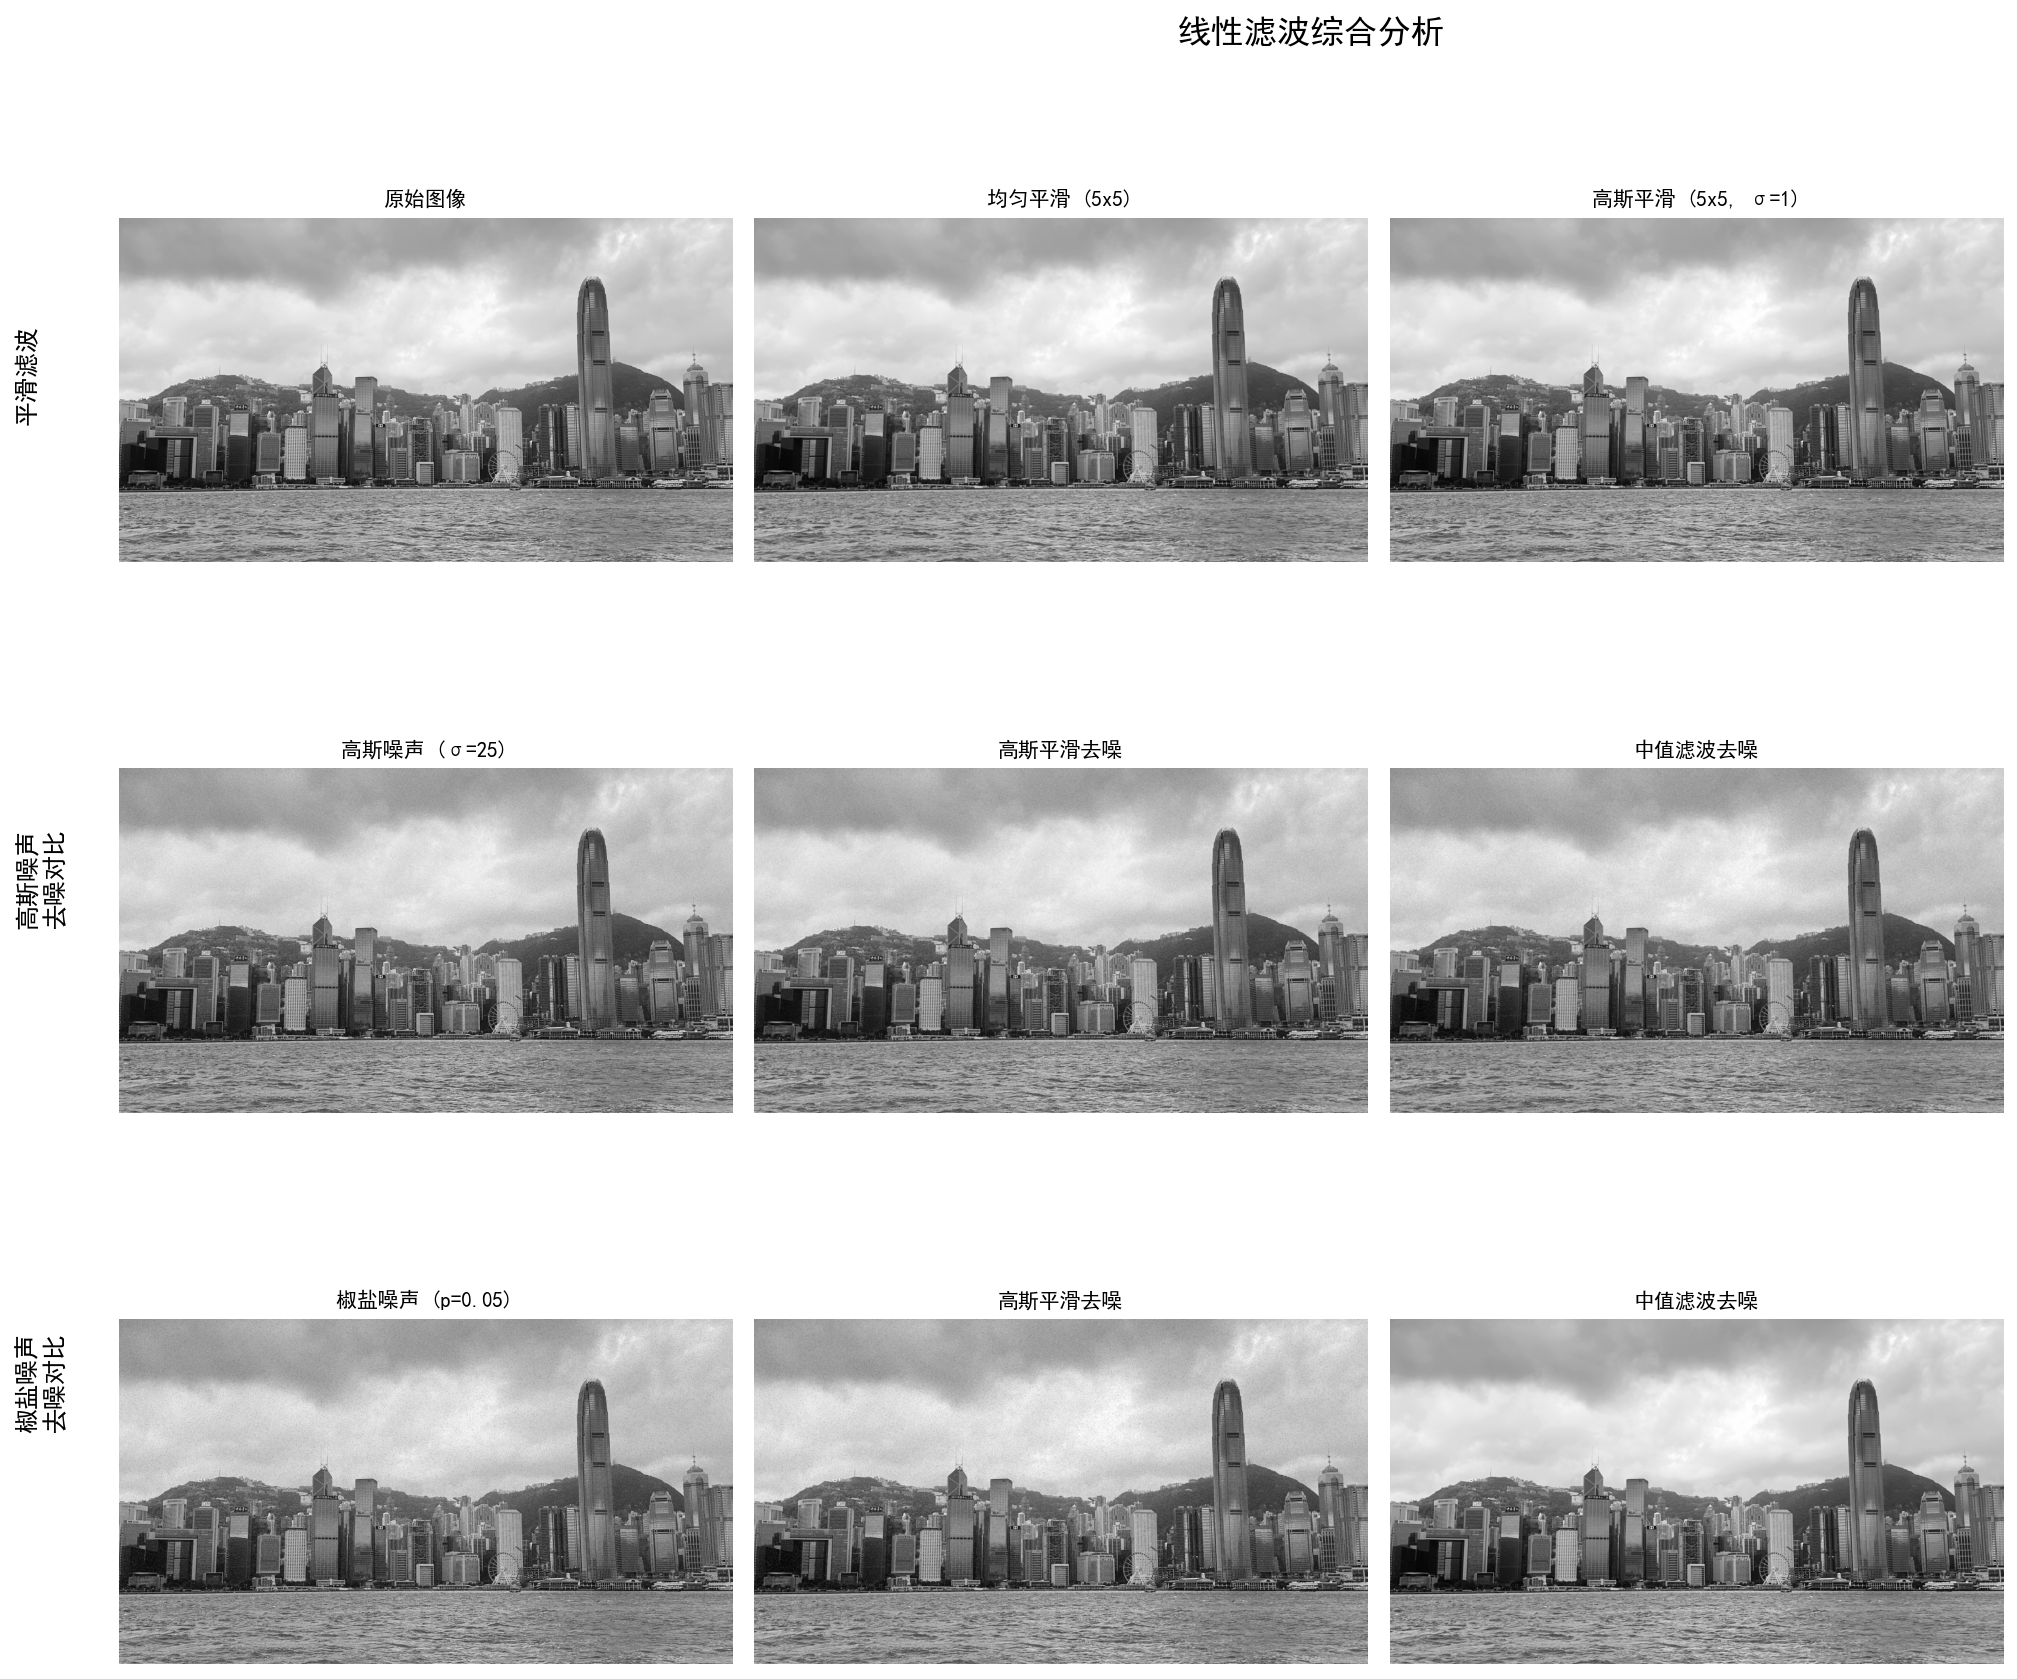
\includegraphics[width=\textwidth]{output_5_analysis.png}
    \caption{线性滤波综合分析（3行$\times$4列子图）}
    \label{fig:analysis}
\end{figure}

图 \ref{fig:analysis} 将所有实验结果整合到一张 3$\times$4 布局的大图中，便于跨方法、跨噪声类型的系统对比。第一行展示平滑滤波的基线效果，第二行和第三行分别展示高斯噪声和椒盐噪声的去噪对比。第 3 列故意留空，在视觉上将"平滑"与"去噪"两组实验分隔开来。

\newpage

% ==================== 第五章：讨论 ====================
\section{讨论}

\subsection{线性 vs 非线性滤波}

本实验最核心的发现是线性滤波与非线性滤波在适用场景上的根本差异：

\begin{table}[H]
    \centering
    \caption{滤波器适用性对比}
    \begin{tabular}{lcc}
        \toprule
        \textbf{滤波器} & \textbf{高斯噪声} & \textbf{椒盐噪声} \\
        \midrule
        高斯平滑（线性） & 好 & 差（产生伪影） \\
        中值滤波（非线性） & 一般 & 优秀 \\
        \bottomrule
    \end{tabular}
\end{table}

这一差异来源于两类滤波器的数学本质：
\begin{itemize}[leftmargin=*]
    \item \textbf{线性滤波}对所有像素一视同仁地加权平均——在噪声普遍存在时（高斯噪声）有效降低方差，但在仅有少数极端噪声时（椒盐噪声），极端值会污染整个邻域。
    \item \textbf{非线性滤波}通过排序操作选择性忽略极端值——对脉冲噪声天然免疫，但在噪声普遍存在时无法区分信号与噪声。
\end{itemize}

\subsection{噪声抑制与边缘保留的权衡}

所有空间域滤波都面临一个根本性的权衡（trade-off）：更大的核 = 更强的去噪能力 + 更严重的边缘模糊。这一现象的数学解释为：

\begin{itemize}[leftmargin=*]
    \item 对于线性滤波，核大小 $K$ 与噪声方差缩减比例为 $1/K^2$，但同时核的"空间扩散"范围也以 $O(K^2)$ 增长，导致跨边缘污染加剧。
    \item 中值滤波在此权衡上表现更好——因为中位数操作具有"边缘保持"（edge-preserving）特性，只要边缘两侧像素在邻域中各占一半以上，中位数就不会跨过边缘。
\end{itemize}

实际应用中，通常需要根据噪声类型和图像内容选择合适的滤波器及参数。更高级的方法（如双边滤波 Bilateral Filter、非局部均值 NLM、BM3D）在噪声抑制和边缘保留之间取得了更好的平衡，但计算复杂度相应增加。

\subsection{参数敏感性分析}

\begin{itemize}[leftmargin=*]
    \item \textbf{高斯噪声 $\sigma$：}$\sigma$ 越大，噪声越强，去噪难度越大。$\sigma=25$ 为中等水平，$\sigma>50$ 时高斯平滑仍有效但需增大核大小（如 $7\times7$ 或 $9\times9$）。
    \item \textbf{椒盐噪声 $p$：}$p$ 越大，噪声密度越高。中值滤波在 $p<0.5$ 时理论上有良好的去噪效果（因为"好"像素仍占多数），但 $p$ 接近 0.5 时性能急剧下降。本实验的 $p=0.05$ 在 $5\times5$ 核（25 个像素）下最多期望覆盖 1--2 个噪点，中值滤波能轻松处理。
    \item \textbf{核大小 $K$：}$K=5$ 是平滑与细节保留之间的折中选择。$K=3$ 去噪不足，$K=7$ 过度平滑。
\end{itemize}

\subsection{实验局限与改进方向}

\begin{enumerate}[leftmargin=*]
    \item \textbf{客观评价指标缺失：}本实验仅采用主观视觉评价，未使用 PSNR（峰值信噪比）或 SSIM（结构相似性）等定量指标。在有原始无噪声图像（ground truth）的情况下，可使用 PSNR 和 SSIM 实现客观的数值对比。
    \item \textbf{参数范围有限：}仅测试了单一参数组合（$\sigma=25$, $p=0.05$, $K=5$），未进行系统的参数扫描实验。
    \item \textbf{滤波器种类有限：}未纳入自适应中值滤波、双边滤波等更先进的去噪方法作为对比基线。
    \item \textbf{单张测试图像：}仅使用一张照片，未考察滤波器在不同图像内容（纹理丰富 vs 平坦、高对比度 vs 低对比度）下的表现差异。
\end{enumerate}

\newpage

% ==================== 第六章：总结 ====================
\section{总结}

本实验通过 Python + OpenCV 实现了图像线性滤波的完整流程，涵盖了高斯金字塔构建、噪声生成、空间域平滑滤波和去噪处理五大模块，并使用真实照片进行了系统的对比实验。

\textbf{核心发现：}

\begin{enumerate}[leftmargin=*]
    \item 高斯金字塔通过反复的高斯平滑 + 下采样实现多尺度表示，每层分辨率减半，信息量逐层递减。
    \item 高斯噪声（加性噪声）和椒盐噪声（脉冲噪声）是两种完全不同的退化模型：前者影响所有像素（幅度分布），后者仅影响少数像素（空间随机）。
    \item 线性滤波器（均匀平滑、高斯平滑）能有效抑制高斯噪声（方差降低 $1/K^2$），但对椒盐噪声无效，甚至因"涂抹"噪点而产生视觉伪影。
    \item 非线性中值滤波对椒盐噪声有卓越的去噪效果——利用排序操作将极端值天然排斥在中位数之外，同时保持边缘锐利。
    \item 空间域滤波的核心挑战是"噪声抑制 vs 边缘保留"的权衡——所有方法都在这两个目标之间寻求平衡，不存在普适的最优解。
\end{enumerate}

本实验为后续学习更高级的图像处理技术（如频域滤波、小波去噪、深度学习去噪）奠定了理论与实验基础。

\newpage

% ==================== 附录 ====================
\appendix
\section{完整源代码 (main.py)}

以下为实验完整源代码，包含所有模块的实现与注释。

\lstinputlisting[caption={main.py —— 线性滤波实验完整代码}, label=lst:fullcode, lastline=277]{main.py}

\section{输出文件清单}

\begin{table}[H]
    \centering
    \caption{实验输出文件}
    \begin{tabular}{lll}
        \toprule
        \textbf{文件名} & \textbf{内容} & \textbf{格式} \\
        \midrule
        \texttt{output\_1\_pyramid.png} & 4层高斯金字塔 & 1276$\times$3408, 灰度 \\
        \texttt{output\_2\_noise.png} & 原始图像 + 两种噪声对比 & 1276$\times$3828, 灰度 \\
        \texttt{output\_3\_smoothing.png} & 原始 + 均匀平滑 + 高斯平滑 & 1276$\times$3828, 灰度 \\
        \texttt{output\_4\_denoising.png} & 2$\times$3 去噪对比矩阵 & 2552$\times$3828, 灰度 \\
        \texttt{output\_5\_analysis.png} & 3$\times$4 综合分析大图 & 3828$\times$5104, 灰度 \\
        \bottomrule
    \end{tabular}
\end{table}

\section{运行说明}

在项目目录下执行以下命令即可复现所有实验结果：

\begin{lstlisting}[language=bash, caption={运行命令}]
pip install -r requirements.txt
python main.py input_photo.jpg
\end{lstlisting}

若需使用其他图像，将 \texttt{input\_photo.jpg} 替换为目标图像路径即可。生成的 5 张 PNG 输出图将保存在当前目录。

\end{document}
